\documentclass[10pt,portuguese]{article}

\usepackage{fourier}

\usepackage[]{graphicx}
\usepackage[]{color}
\usepackage{xcolor}
\usepackage{alltt}
\usepackage{listings}
\usepackage[T1]{fontenc}
\usepackage[utf8]{inputenc}
\setlength{\parskip}{\smallskipamount}
\setlength{\parindent}{5ex}
\usepackage{indentfirst}
\usepackage{listings}
\usepackage{setspace}
\usepackage{hyperref}
\definecolor{blue(munsell)}{rgb}{0.0, 0.5, 0.69}
\hypersetup{
    colorlinks=true,
    linkcolor=blue,
    filecolor=magenta,      
    urlcolor=blue, urlsize=2em
}

% Set page margins
\usepackage[top=100pt,bottom=100pt,left=68pt,right=66pt]{geometry}

% Package used for placeholder text
\usepackage{lipsum}

% Prevents LaTeX from filling out a page to the bottom
\raggedbottom


\usepackage{fancyhdr}
\fancyhf{} 
\fancyfoot[C]{\thepage}
\renewcommand{\headrulewidth}{0pt} 
\pagestyle{fancy}

\usepackage{titlesec}
\titleformat{\chapter}
   {\normalfont\LARGE\bfseries}{\thechapter.}{1em}{}
\titlespacing{\chapter}{0pt}{50pt}{2\baselineskip}

\usepackage{float}
\floatstyle{plaintop}
\restylefloat{table}

\usepackage[tableposition=top]{caption}



\frontmatter

\definecolor{light-gray}{gray}{0.95}

\renewcommand{\contentsname}{Índice}

\begin{document}

\selectlanguage{portuguese}

\begin{titlepage}
	\clearpage\thispagestyle{empty}
	\centering
	\vspace{2cm}
	{\Large\underline{Computação Distribuída} \par}
	\vspace{0.5cm}
	{\small Diogo Nuno Pereira Gomes \par José Nuno Panelas Nunes Lau  \par}
	\vspace{4cm}
	{\LARGE \textbf{Distributed Object Detection}} \\ \vspace{0.5cm}
	\vspace{5cm}
	{\normalsize Hugo Paiva, 93195
	        \\Carolina Araújo, 93248 \par}
	\vspace{2cm}
    
\includegraphics[scale=0.20]{logo_ua.png}
    \vspace{2cm}
	{\normalsize \\DETI \\Universidade de Aveiro \par}
	{\normalsize 25-06-2020 \par}
	\vspace{2cm}
	\pagebreak
\end{titlepage}

\newpage
\section{Introdução}
\par Este trabalho visa a criação de um sistema distribuído de deteção de objetos, sendo necessário estabelecer comunicação entre \textit{workers} e o servidor, concebido com base na \textit{framework} \textit{Flask}, e entre este e os clientes. Apresentar-se-ão, então, as escolhas tomadas relativamente aos protocolos de comunicação em prol do funcionamento do sistema e quais as razões que levaram às mesmas.

\section{Protocolo}
    \begin{figure}[!h]
        \centering
        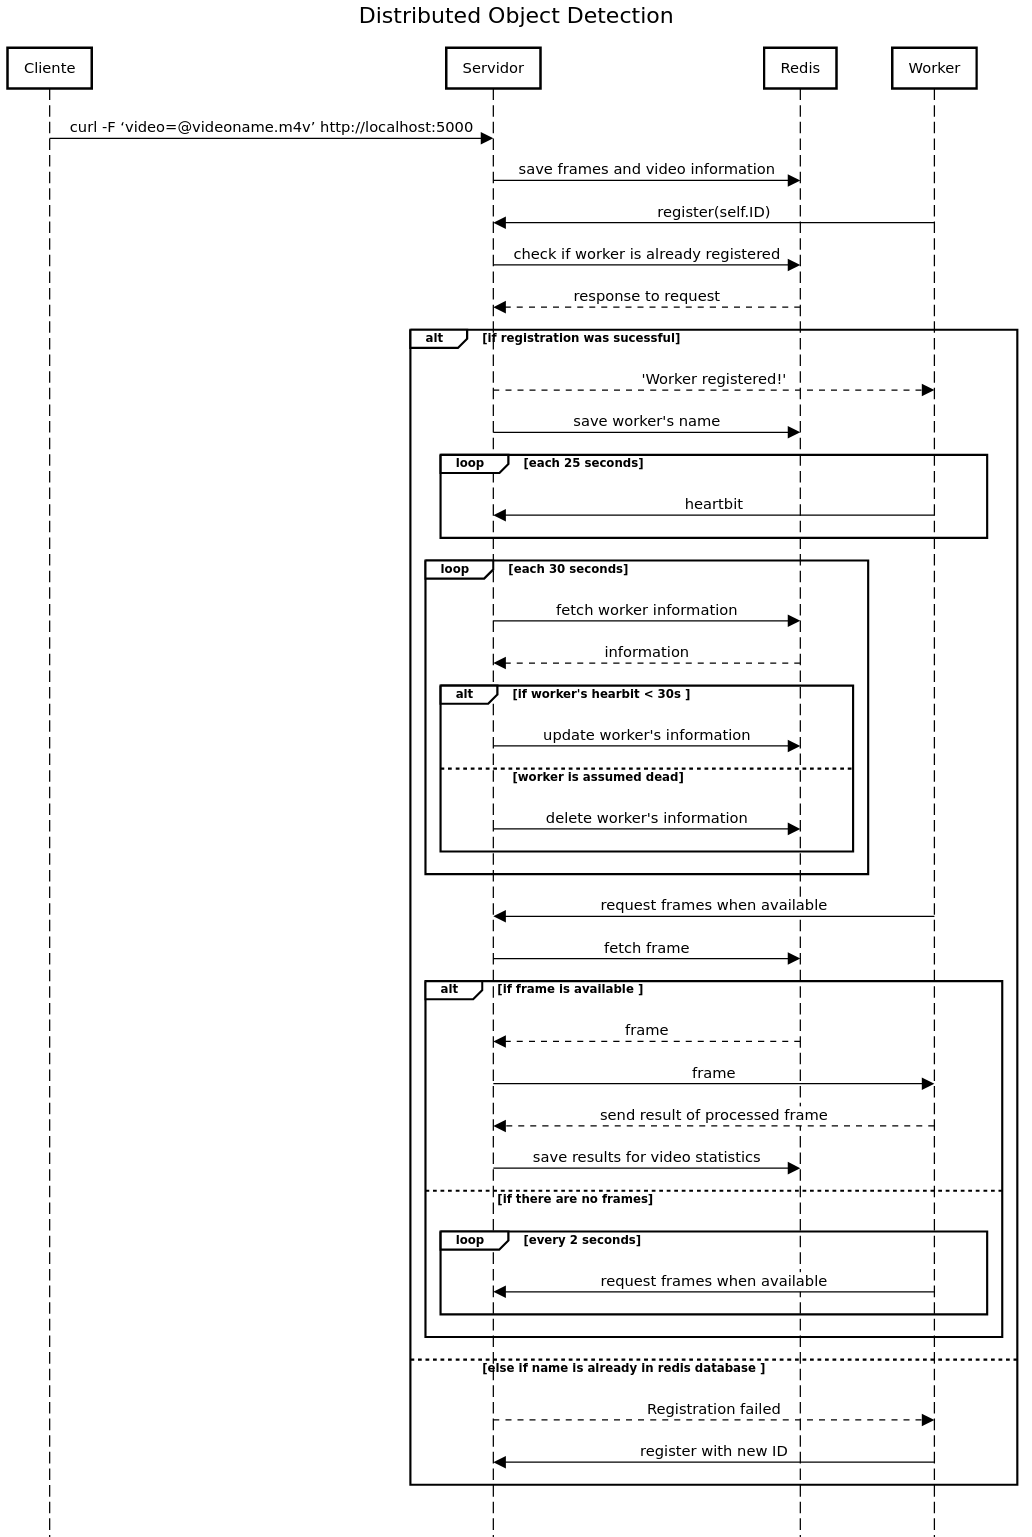
\includegraphics[width=291]{Diagrama.png}
        \caption{Message Sequence Chart entre as 3 entidades e o Redis} 
    \end{figure}
\pagebreak
\par A figura acima retrata o fluxo das mensagens principais trocadas entre as várias entidades que constituem o sistema. 
\par O \textit{cliente} terá de enviar um vídeo para que o servidor possa dividir o mesmo em \textit{frames}. Entretanto, espera-se que os \textit{workers} se registem no servidor para poderem receber tarefas, só depois poderão realmente trabalhar. O servidor comunica maioritariamente com o \textit{Redis}, verificando, introduzindo ou indo buscar dados à base de dados para todas as funções que realiza. 
\par A cada 25 segundos, o \textit{worker}, depois de registado, enviará um \textit{heartbit}, a partir do qual informa o servidor de que ainda se encontra ativo. Já o servidor, a cada 30 segundos, verifica todos os \textit{workers}, eliminando aqueles que se consideram mortos.
\par Paralelamente, os \textit{workers} estão constantemente a pedir \textit{frames} para processar. Caso haja, ser-lhes-á enviada a mesma e eles devolverão o resultado, se não forem mortos entretanto; caso contrário, apenas repetem o \textit{request} dentro de 2 segundos. 

\subsection{Estrutura de Dados}

\par De modo a permitir que o servidor seja executado por múltiplos processos, ou até mesmo existirem múltiplos servidores com endereços diferentes, todos os dados necessários para a execução do mesmo são guardados com recurso a \textbf{\textit{Redis}}, uma base de dados não relacional que guarda os dados na memória principal e que permite o armazenamento de dados de texto ou binários até 512\textit{mb}, cumprindo todos os nossos requisitos. Desta forma, o acesso aos dados continua extremamente rápido.

\par Para armazenar os dados, foram utilizados os seguintes tipos de dados do \textit{Redis}:

 \begin{itemize}
     \item \textbf{Strings} - Utilizado para guardar informações de um vídeo e \textit{worker} após codificação em \textit{JSON}
     \item \textbf{Lists} - Permitiu o armazenamento dos \textit{paths} de cada frame e o \textit{MD5} correspondente ao seu vídeo, também com codificação em \textit{JSON}, e os diversos vídeos que ainda necessitam de processamento (para o \textit{Load Balancer})
     \item \textbf{Sets} - Para guardar os nomes dos diferentes \textit{workers}, não permitindo duplicação em termos de nomes
 \end{itemize}
 
\subsection{Server}
\par É função do servidor gerir todos os \textit{workers} que se encontram ativos, atribuindo \textit{frames} aos mesmos quando estes se mostram disponíveis para tal. Para além disto, deve ainda processar toda a informação vinda dos \textit{workers} referente às diferentes \textit{frames} dos vários vídeos, para poder alertar a presença excessiva de pessoas e, no final, apresentar as estatísticas de cada vídeo. O servidor pode receber vídeos diferentes de vários clientes, sendo sua função dividi-los depois em \textit{frames}.

\subsubsection{Receção e Processamento de Vídeos}
\par A receção de um vídeo é feita utilizando o \textit{endpoint \textbf{/}} onde são feitas algumas verificações como a confirmação da extensão do ficheiro, sendo que apenas é suportado \textit{.mp4} e \textit{.m4v}, e a validação da existência de um ficheiro.

\par Passando estas verificações, é criado um ficheiro temporário utilizando a biblioteca \textit{tempfile} onde é guardado o vídeo recebido para posteriormente ser processado. O processamento foi realizado com recurso a \textit{daemon threads}, algo necessário para garantir a execução do servidor em pleno e para que sejam terminadas juntamente com este, caso seja necessário.

\par No início do processamento, é gerada uma \textit{MD5 hash} do vídeo com o objetivo de o identificar indubitavelmente. Assim, caso um vídeo igual esteja a ser processado ou já tenha sido processado, o servidor não necessita de lidar com o que acabou de chegar, imprimindo na consola os resultados, caso o outro vídeo igual já tenha impresso anteriormente. 
Como referido anteriormente, o processamento do vídeo gera as várias \textit{frames} deste, guardando na base de dados  \textit{Redis} o \textit{path} do ficheiro temporário onde se encontram as diferentes frames. No final da divisão em \textit{frames}, são também guardadas na base de dados as informações do vídeo e, posteriormente, colocando-o em lista de espera para os \textit{workers} começarem a trabalhar.

\subsubsection{Envio de Frames aos Workers}
\par Acedendo ao \textit{endpoint \textbf{/worker/<name>/request}}, será atribuída, ao respetivo worker, uma frame, caso ainda exista alguma por processar.
\par O servidor recorre à lista de vídeos por processar, guardada no \textit{Redis}, para ir buscar o identificador de um vídeo que ainda não tenha tido as suas \textit{frames} processadas na totalidade, retirando o \textit{md5} do vídeo que esteja na cabeça da lista. A partir do \textit{md5}, irá buscar a \textit{frame}, também na cabeça da lista de \textit{frames} desse vídeo, que será então retornada. É, portanto, atualizada a informação, \textit{heartbit} e \textit{frame} atual, do próprio \textit{worker}. 
\par Feito isto, se depois da atribuição ainda houver mais \textit{frames} para processar relativas ao vídeo em questão, voltará a colocar-se o identificador desse mesmo vídeo no fim da lista de vídeos por processar. Deste modo, garante-se o processamento de vídeos em concorrência, sendo que um vídeo nunca tem de esperar que outro acabe de processar totalmente para chegar a sua vez na lista.

\subsubsection{Receção dos Resultados dos Workers}
\par Cada vez que um \textit{worker} acaba de processar a \textit{frame} que lhe foi atribuída, acede ao \textit{endpoint \textbf{/worker/<name>/result}}.

\par O servidor liberta a \textit{frame} associada ao \textit{worker}, para que, caso esse mesmo \textit{worker} morra, a \textit{frame} não seja atribuída a um outro, visto que já foi processada. De seguida, o servidor guarda numa lista do \textit{Redis} os resultados para posteriormente serem processados durante a execução de uma \textit{daemon thread}. Esta vai buscar a informação armazenada relativa ao vídeo a que a \textit{frame} pertence e, também, a informação enviada pelo \textit{worker}. 
\par É atualizada toda a informação, desde o tempo total de processamento do vídeo, o número de \textit{frames} já processadas, bem como a contagem de todas as entidades que foram detetadas. Caso o número de pessoas detetadas exceda o limite estipulado, será impressa o número da \textit{frame} em que tal se sucedeu, bem como a quantidade de pessoas que nela se detetaram. 
\par Em termos da informação impressa perante a entrega dos resultados da última \textit{frame} de um vídeo, são apresentadas as estatísticas que os docentes solicitaram. 

\subsubsection{Manutenção dos Workers ativos}
\par Em qualquer uma das interações entre servidor e \textit{worker}, o servidor atualiza a informação que mantém sobre esse mesmo, para poder, periodicamente, verificar se ele ainda se encontra ativo. No entanto, os próprios \textit{workers} acedem, também de modo periódico (a cada 25 segundos), ao \textit{endpoint \textbf{/worker/<name>/alive}}, para manifestar ao servidor que ainda se encontram vivos. 
\par Na função \textit{\textbf{main}}, ao ser iniciado o servidor, corre-se pela primeira vez a função \textit{\textbf{checkWorkers()}} que, desde então, de 30 em 30 segundos, iniciará uma \textit{thread} cuja função é percorrer a lista de \textit{workers} que se consideram ativos e verificar se isso é ainda, de facto, verdade. 
\par Quando o \textit{worker} se regista com sucesso, é adicionado o seu nome ao \textit{Set} de \textit{workers}, e embora não lhe seja automaticamente atribuída uma \textit{frame}, é atribuído o primeiro \textit{heartbit}, \textit{i.e}, a hora a que o registo sucedeu, sendo então guardada a informação na base de dados. A partir daí, cada vez que a \textit{thread} é chamada, o servidor verifica se, entre a última hora associada a cada \textit{worker} e a hora atual, passaram 30 segundos. Se sim, assume-se que o \textit{worker} morreu e a \textit{frame} que lhe estava associada é colocada novamente na lista de \textit{frames} por processar, mas no início da mesma, uma vez que era suposto já ter sido processada e tem, portanto, mais prioridade. De seguida, apagar-se-ão referências a esse \textit{worker} na base de dados . 

\subsection{Worker}
\par O \textit{worker} é uma entidade cujas únicas funções, após um contacto inicial com o servidor, são obter \textit{frames}, processá-las, devolver os resultados e manter a comunicação com o servidor ativa.

\subsubsection{Registo no Servidor}
\par Ao executar o \textit{worker}, este regista-se no servidor de modo a dar-se a conhecer para permitir a sua tolerância a falhas. Para este registo, é gerado um identificador com o comprimento de 8 caracteres, contendo letras e números aleatórios. Caso, mesmo assim, o identificador já estiver registado no servidor, este gera novamente um novo e tenta realizar novamente o registo ao fazer um pedido \textit{GET} ao \textit{endpoint \textbf{/worker/<name>}}.

\subsubsection{Processamento de Frames e Envio dos Resultados}
\par Após o registo com sucesso do \textit{worker}, este faz pedidos de \textit{frames} para processar à medida que esteja disponível. Para isso, são feitos pedidos \textit{GET} ao \textit{endpoint \textbf{/worker/<name>/request}}, os quais são respondidos com o ficheiro correspondente ao \textit{path} guardado em \textit{Redis}, que contém a \textit{frame} que irão processar. Com isto, o \textit{worker} gera os resultados, enviando-os ao servidor através de um pedido \textit{POST}. 
\par Caso o \textit{worker} tenha sido considerado morto pelo servidor, este volta a efetuar o registo, de modo a conseguir pedir novas \textit{frames} para processar. Se porventura o servidor não tiver \textit{frames} para processamento, o \textit{worker} espera 2 segundos para voltar a efetuar o mesmo pedido, repetindo-se a mesma sequência até existir conteúdo para trabalhar.
\par Para tornar o processamento o mais rápido possível, passou-se a criação do modelo \textit{keras} e a leitura dos pesos para o \textit{scope} global, tendo assim de serem realizados apenas uma vez. 

\subsubsection{Heartbit}
\par Do mesmo modo que o servidor, o \textit{worker} irá chamar periodicamente uma função, depois de se registar com sucesso, que informa, através do \textit{endpoint \textbf{/worker/<name>/alive}}, que ainda se encontra ativo.
\par Isto deve-se ao facto de, caso o \textit{worker} tenha sido morto ou tenha sofrido \textit{crash}, a \textit{frame} que lhe estava atribuída tem de ser atribuída a um outro, para que o processamento dos vídeos se mantenha coerente e breve.
\par Chamando uma \textit{thread} para realizar o envio do \textit{heartbit}, mesmo que o \textit{worker} esteja, de momento, a demorar demasiado tempo a processar a \textit{frame}, é possível avisar o servidor de que ele ainda se encontra ativo.

\section{Estratégia de Validação da Solução}

\par Os testes que foram feitos à medida que o projeto ia sendo construído permitiram que o grupo detetasse certas situações que foram então tratadas, como por exemplo: lidar com os casos de tentativas de acesso por parte de \textit{workers} quando o servidor não está ativo, registos falhados, parâmetros incorretos no \textit{curl}, \textit{endpoints} não existentes, ficheiros de tipos inválidos, tentativa de registos sob um nome já existente, \textit{etc}.
\par Para correr a solução criada, deve-se instalar o \textit{Redis}, seguindo os comandos de instalação do \textit{README.txt}.
\subsection{Resultados}
\par O Total Time nos \textit{screenshots} abaixo contabiliza o tempo desde que se envia o vídeo para o server até os resultados finais serem impressos. 
    \begin{figure}[!h]
        \centering
        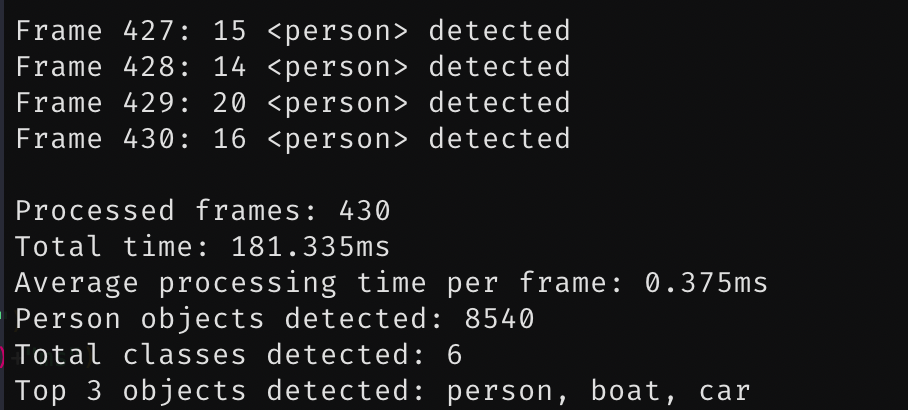
\includegraphics[width=0.7\textwidth]{1worker.png}
        \caption{Resultados do processamento do vídeo moliceiros.m4v com 1 \textit{worker}} 
    \end{figure}
    
    \begin{figure}[!h]
        \centering
        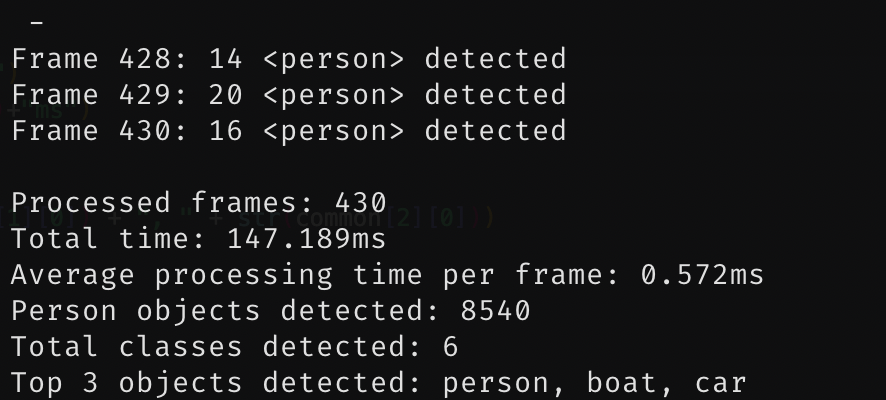
\includegraphics[width=0.7\textwidth]{2workers.png}
        \caption{Resultados do processamento do vídeo moliceiros.m4v com 2 \textit{workers}} 
    \end{figure}
    
    \begin{figure}[!h]
        \centering
        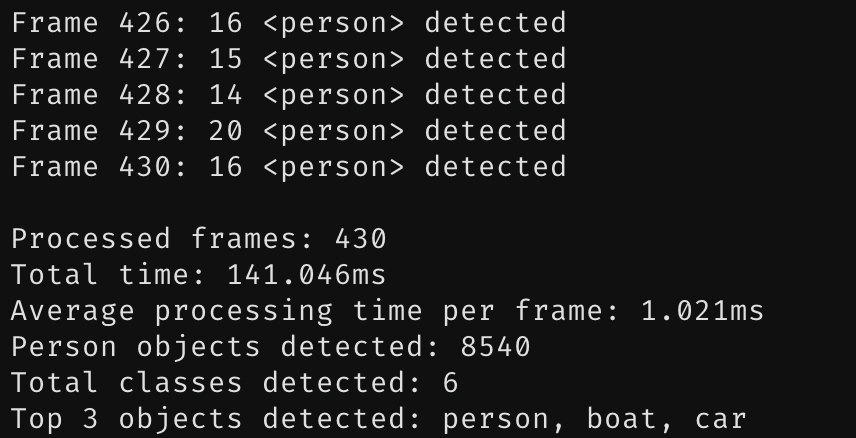
\includegraphics[width=0.7\textwidth]{4workers.png}
        \caption{Resultados do processamento do vídeo moliceiros.m4v com 4 \textit{workers}} 
    \end{figure}
\newpage
\section{Conclusão}
\par De modo geral, considera-se que a solução criada cumpre todos os requisitos propostos e, até os ultrapassa em algumas situações, como no caso da utilização de um identificador \textit{MD5 Hash}. 
\par Entre as dificuldades encontradas aquando da realização do projeto, está o facto de inicialmente se ter criado um cliente que dividia ele mesmo as \textit{frames}, enviando-as então para o servidor, em vez de um simples \textit{curl}. Isto ocorreu devido a um mal entendido sobre qual o propósito do servidor, tendo-se pensado que se o cliente fizesse a divisão em \textit{frames} dos vídeos, se aliviava carga do servidor, o que por sua vez acelerava o tratamento do vídeo. 
\par Para além disso, inicialmente também foi morosa a pesquisa de quais as ferramentas que se pretendia utilizar, bem como definir a estratégia de comunicação, em prol de um processamento rápido que, ao mesmo tempo, permitisse uma boa gestão dos recursos. Julga-se que as ferramentas utilizadas são aptas para a o objetivo deste trabalho. 

\section{Referências}
    \bibliographystyle{plain}
    
    \bibliography{biblist}
    [1] \url{https://flask.palletsprojects.com/en/1.1.x/}
    \par
    [2] \url{https://redis.io/documentation}
    \par
    [3] \url{https://redis-py.readthedocs.io/en/stable/}
    \par
    [4] \url{https://requests.readthedocs.io/en/master/}
    \par 
    [5] \url{https://docs.python.org/3/library/tempfile.html}
    \par
    [6] \url{https://docs.python.org/3/library/hashlib.html}
    \par
    [7] \url{https://tinyurl.com/y68mthof}

\end{document}

